% !TeX root = ../libro.tex
% !TeX encoding = utf8

\chapter{Conclusiones finales}\label{ch:septimo-capitulo}

\section{Conclusiones finales}
\subsection{Campos magnéticos de intensidad fija vs. variable}
En \cite{Caballero2020} ya abordamos el estudio de la abundancia superficial de litio en el Sol. Aquel trabajo previo sentó las bases para el desarrollo del presente. En él avanzábamos como futuras líneas de investigación un conocimiento más profundo sobre cómo los campos magnéticos están ligados a la rotación y cómo evolucionan en el tiempo. También mostramos cómo ajustando el valor de $\amlt$ podíamos influir en las abundancias de Li. Por tanto, una comparación entre los resultados obtenidos anteriormente y los de este estudio pone en perspectiva las diferencias y similitudes entre ambos estudios, así como los avances realizados desde entonces. La Tabla \ref{tab:caballero2023_2020} resume las principales diferencias entre ambos trabajos, en línea con lo ya avanzado, es decir, incorporamos formalismos que nos permiten evolucionar temporalmente el $B$ y $\amlt$.\par 

\begin{table}
	\centering
	\begin{threeparttable}
		\begin{tabular}{lll} 
			\hline
			Parameter & This work & \cite{Caballero2020}\\
			\hline
			Convection & MLT variable $\alpha_{\textrm{MLT}}$ & MLT fixed $\alpha_{\textrm{MLT}}=1.82$\\
			Overshoot & deactivated & $f_{\textrm{ov,core}}=0.0160$,\\ & & $f_{\textrm{ov,sh}}=0.0174$\\
			Magnetic Braking & \cite{Gallet2013} & \cite{Ud-Doula2008} \\ Formalism & & \\
			Magnetic Field & B(G) variable & B(G) pre-set [3.0G-5.0G]\\ Strength & & \\
			Number of OC's & 64 & 1 \\
			Source of data & GDR3.0 GES DR5.0 & \cite{Sestito2005} \\
			\hline
		\end{tabular}
	\end{threeparttable}
	\caption{Comparison with \cite{Caballero2020} work.}
	\label{tab:caballero2023_2020}
\end{table}

La Figura \ref{fig:li_var_vel_4_0g4} muestra la evolución de la abundancia de Li para $\omegaini$ entre 0.0084 y 0.0336 en presencia de un campo magnético con una intensidad de 4G. Hemos aumentado la versión original con el mismo conjunto de datos OCs recogidos aplicados en este nuevo trabajo, de forma que sea posible una comparación consistente entre ambos formalismos. Si centramos nuestra atención en la simulación con $\omegaini$ = 0.0336, la simulación reproduce A(Li) = 1.024 dex, valor que está en línea tanto con el del Sol (1.1 $\pm$ 0.1 dex) como con los valores obtenidos en la Figura \ref{fig:li_var_vel_var_g_3} del presente trabajo (1.133 dex) para $\omegaini$ = 0.14 y 0.1425. Aunque en este último caso los modelos se inicializaron con valores de $\omegaini$ más altos que en el primero, lo que resulta en $B$ hasta 3 órdenes de magnitud más intensivos ($\approx$ 1KG frente a 4G) la simulación en ambos trabajos acaba produciendo valores muy similares tanto para la velocidad rotacional como para el A(Li). Esto se explica en parte porque una mayor intensidad de campo magnético implica un efecto MB más intenso (véanse las figuras \ref{fig:rot_vel_var_vel_var_g3} y \ref{fig:rot_vel_var_g3}). \& \ref{fig:rot_vel_var_vel_4_0g4}). En el primer caso, el efecto de desaceleración es más agudo que en el segundo, por lo que deja de destruir Li antes.\par

Sin embargo, este efecto no es suficiente para contrarrestar eficazmente la destrucción de Li. El otro elemento decisivo que entra en juego es el valor de $\amlt$. Como se ejemplifica en \cite{Caballero2020} su valor tiene un impacto inversamente proporcional en la destrucción de Li, donde un valor más bajo resultó en una menor destrucción de Li, particularmente durante el PMS. En la figura \ref{fig:alpha_mlt_var_vel_g3} observamos la evolución temporal del valor $\amlt$. Hasta la última fase de la PMS, el valor $\amlt$ es sustancialmente inferior a 1,82, el valor preestablecido e invariante utilizado en nuestro trabajo anterior, lo que se traduce en una menor destrucción de Li y permite al modelo alcanzar la ZAMS con una reserva de Li $\approx$ 29\% dex mayor. Esta mayor reserva de Li compensa la mayor destrucción inducida por los modelos inicializados con $\omegaini$ mayor velocidad angular.\par

Del mismo modo, procedemos a mostrar la evolución de la velocidad de rotación superficial en la Figura \ref{fig:rot_vel_var_vel_4_0g4} y seleccionamos la simulación con $\omegaini$ = 0.0336. De nuevo, los valores similares se explican por la mayor eficiencia del MB en el nuevo modelo. Aunque las simulaciones alcanzan la ZAMS con valores de velocidad de rotación de hasta el 200\% para los modelos inicializados con $\omegaini$ más altos, el campo magnético más intenso produce una desaceleración más pronunciada para el mismo intervalo de tiempo. Este hecho es especialmente notable en el periodo de tiempo comprendido entre la ZAMS y 1 Ga. La velocidad de rotación obtenida en el ecuador de 4.82 km/s, es un valor bastante próximo a 4.72 km/s, es decir, el valor simulado para $\omegaini$ = 0.0336 en la Figura \ref{fig:rot_vel_var_vel_var_g3}.\par

A la vista de los valores obtenidos, podemos concluir que el nuevo modelo introducido en el presente trabajo no sólo es congruente con los resultados de los trabajos en los que se basa, sino también con los de \cite{Caballero2020}. Adicionalmente, esta nueva versión expone la ventaja de no tener que recurrir al uso de unos valores prefijados para $B$ y $\amlt$, y sin recurrir a activar el overshooting. En definitiva, esto representa una mejora significativa y apoya nuestra línea de investigación orientada a evitar valores preestablecidos haciéndolos evolucionar dinámicamente con parámetros solares clave.\par


\begin{figure}
	\centering
	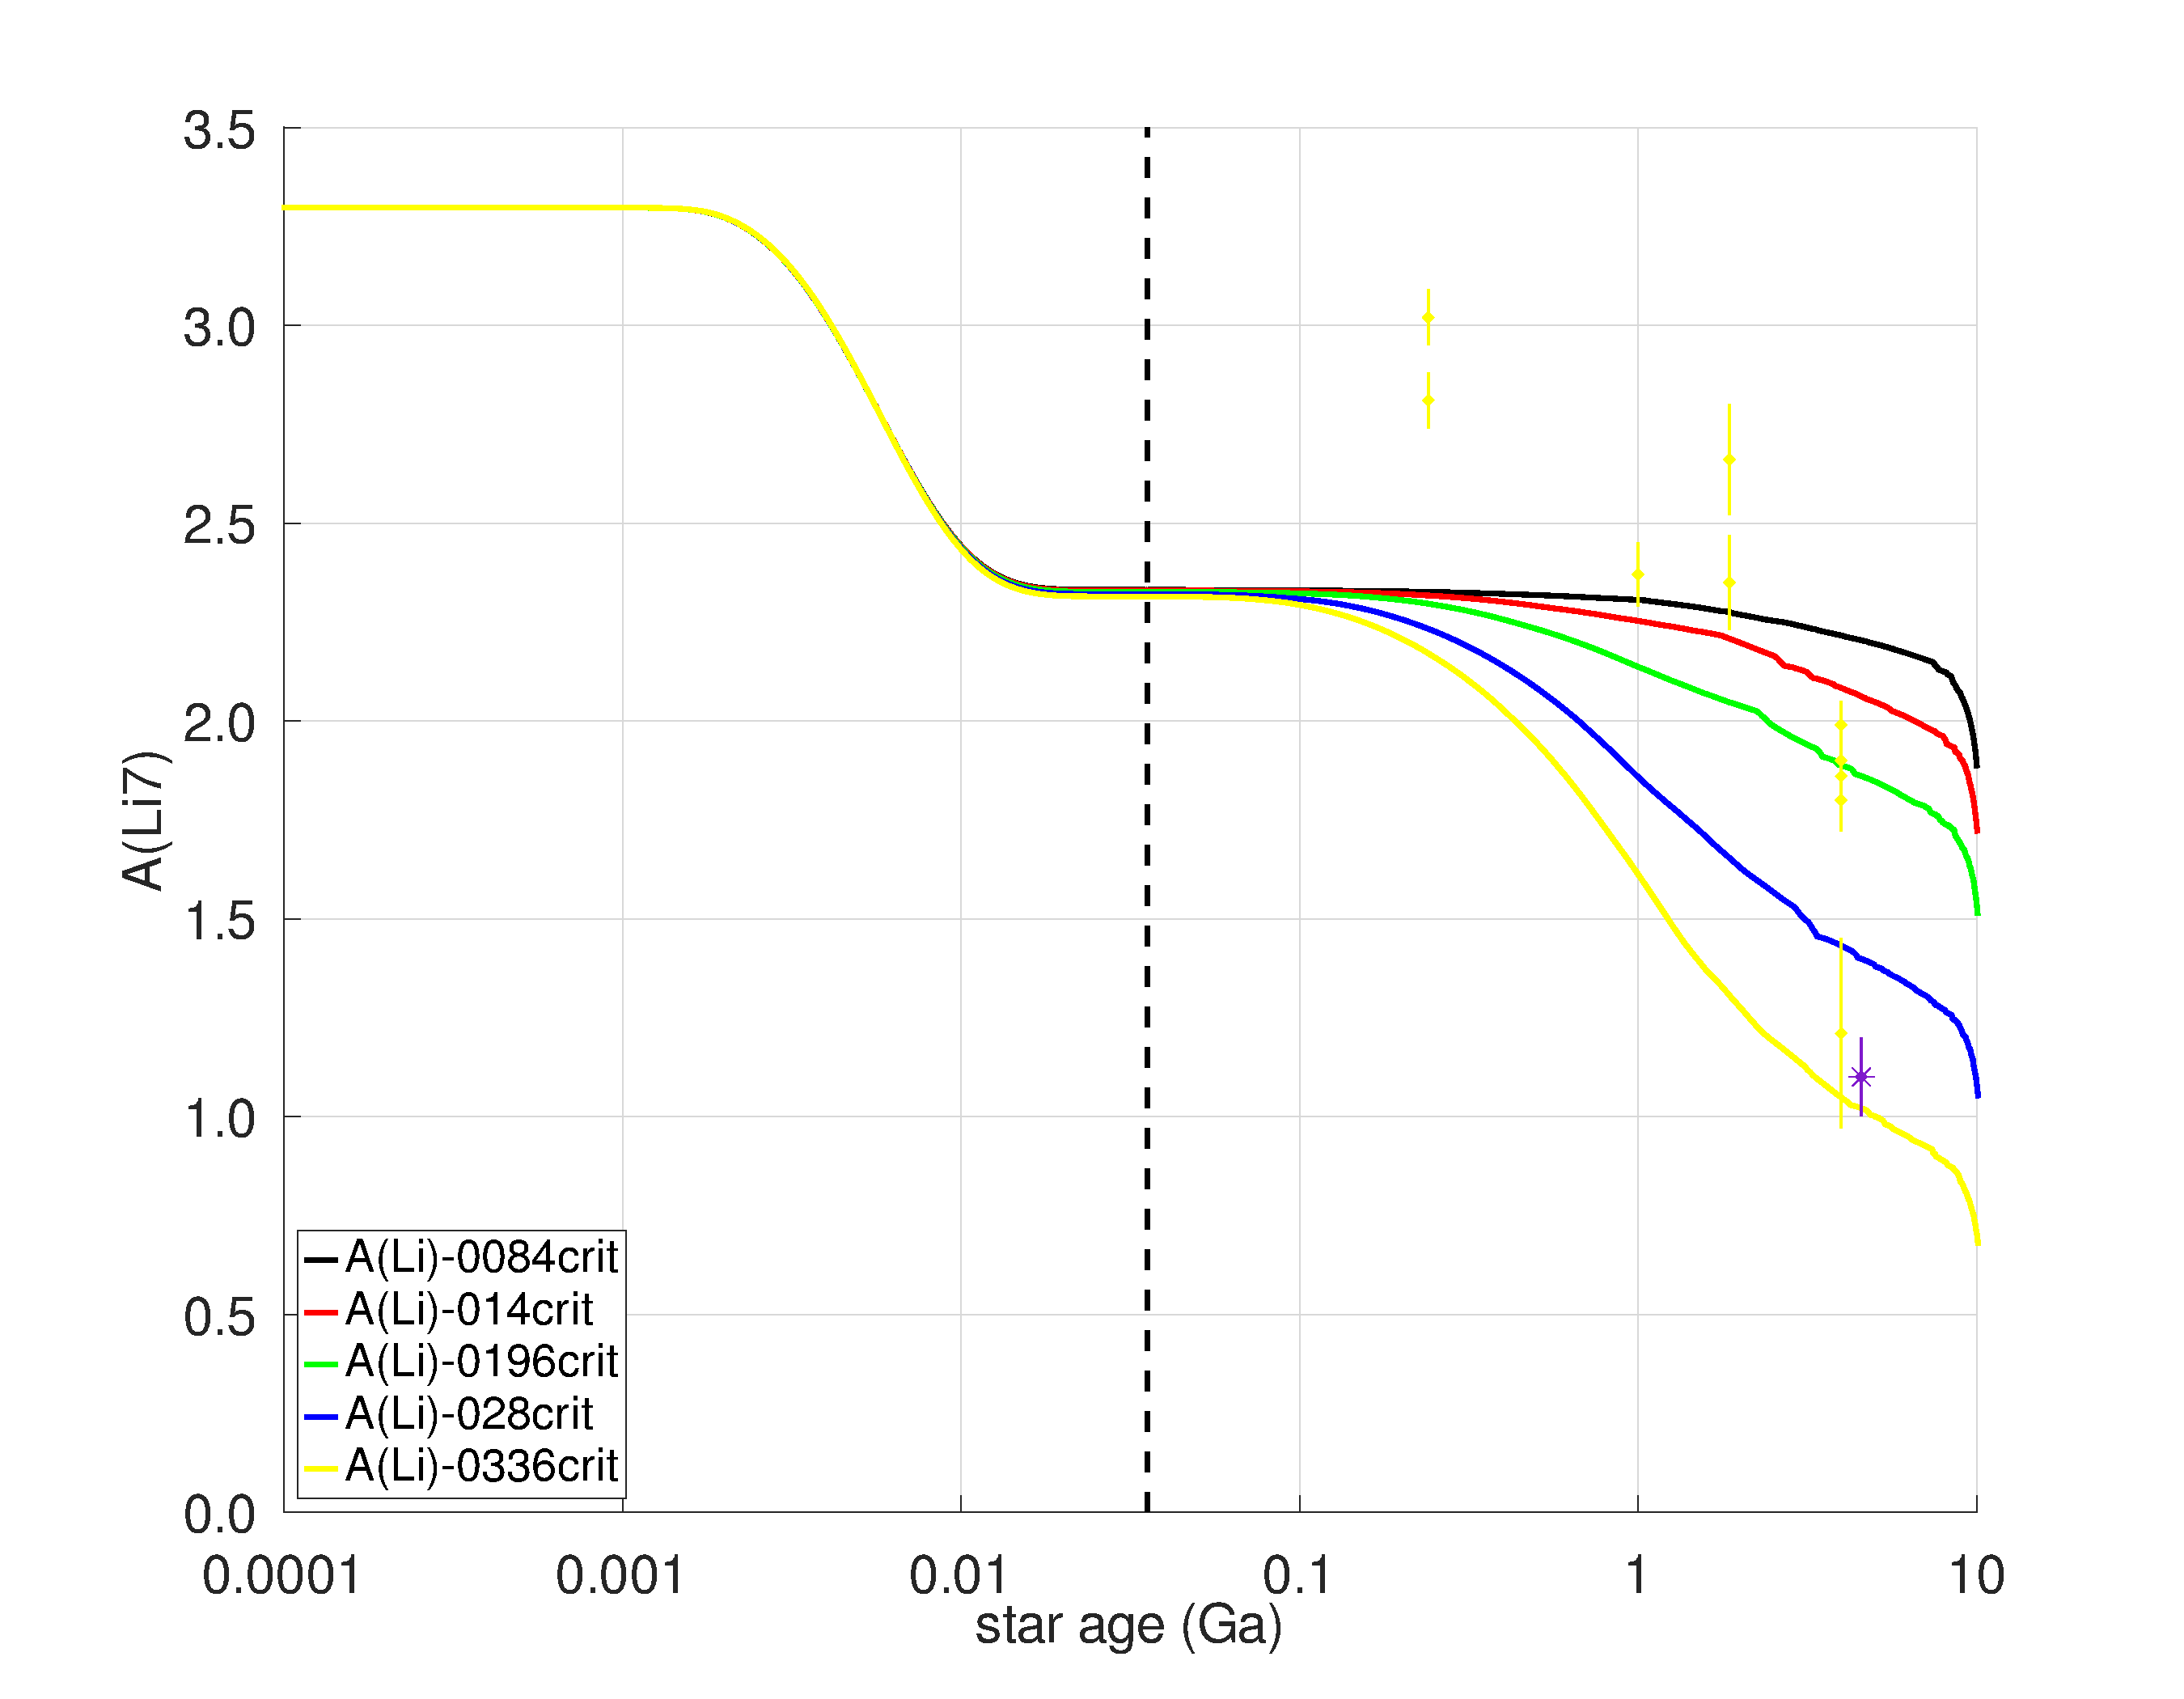
\includegraphics[width=0.7\textwidth]{img/paper2/li_var_vel_4_0g4.pdf}
	\caption{La evolución de la abundancia superficial del \isotope[7]{Li} en relación con el \isotope[1]{H}, en función del tiempo para varios modelos de 1 $\msun$. Los modelos incluyen un campo magnético con una intensidad de 4G. La línea negra continua representa el modelo de referencia según \cite{Choi2016}. El resto de líneas son modelos que incluyen rotación inicial con $\omegaini$ entre 0.0084 y 0.0336, respectivamente. La estrella morada son las abundancias superficiales de Li para el Sol actual \cite{Asplund2009}. La línea vertical discontinua hace referencia a la ZAMS.}
	\label{fig:li_var_vel_4_0g4}
\end{figure}

\begin{figure}
	\centering
	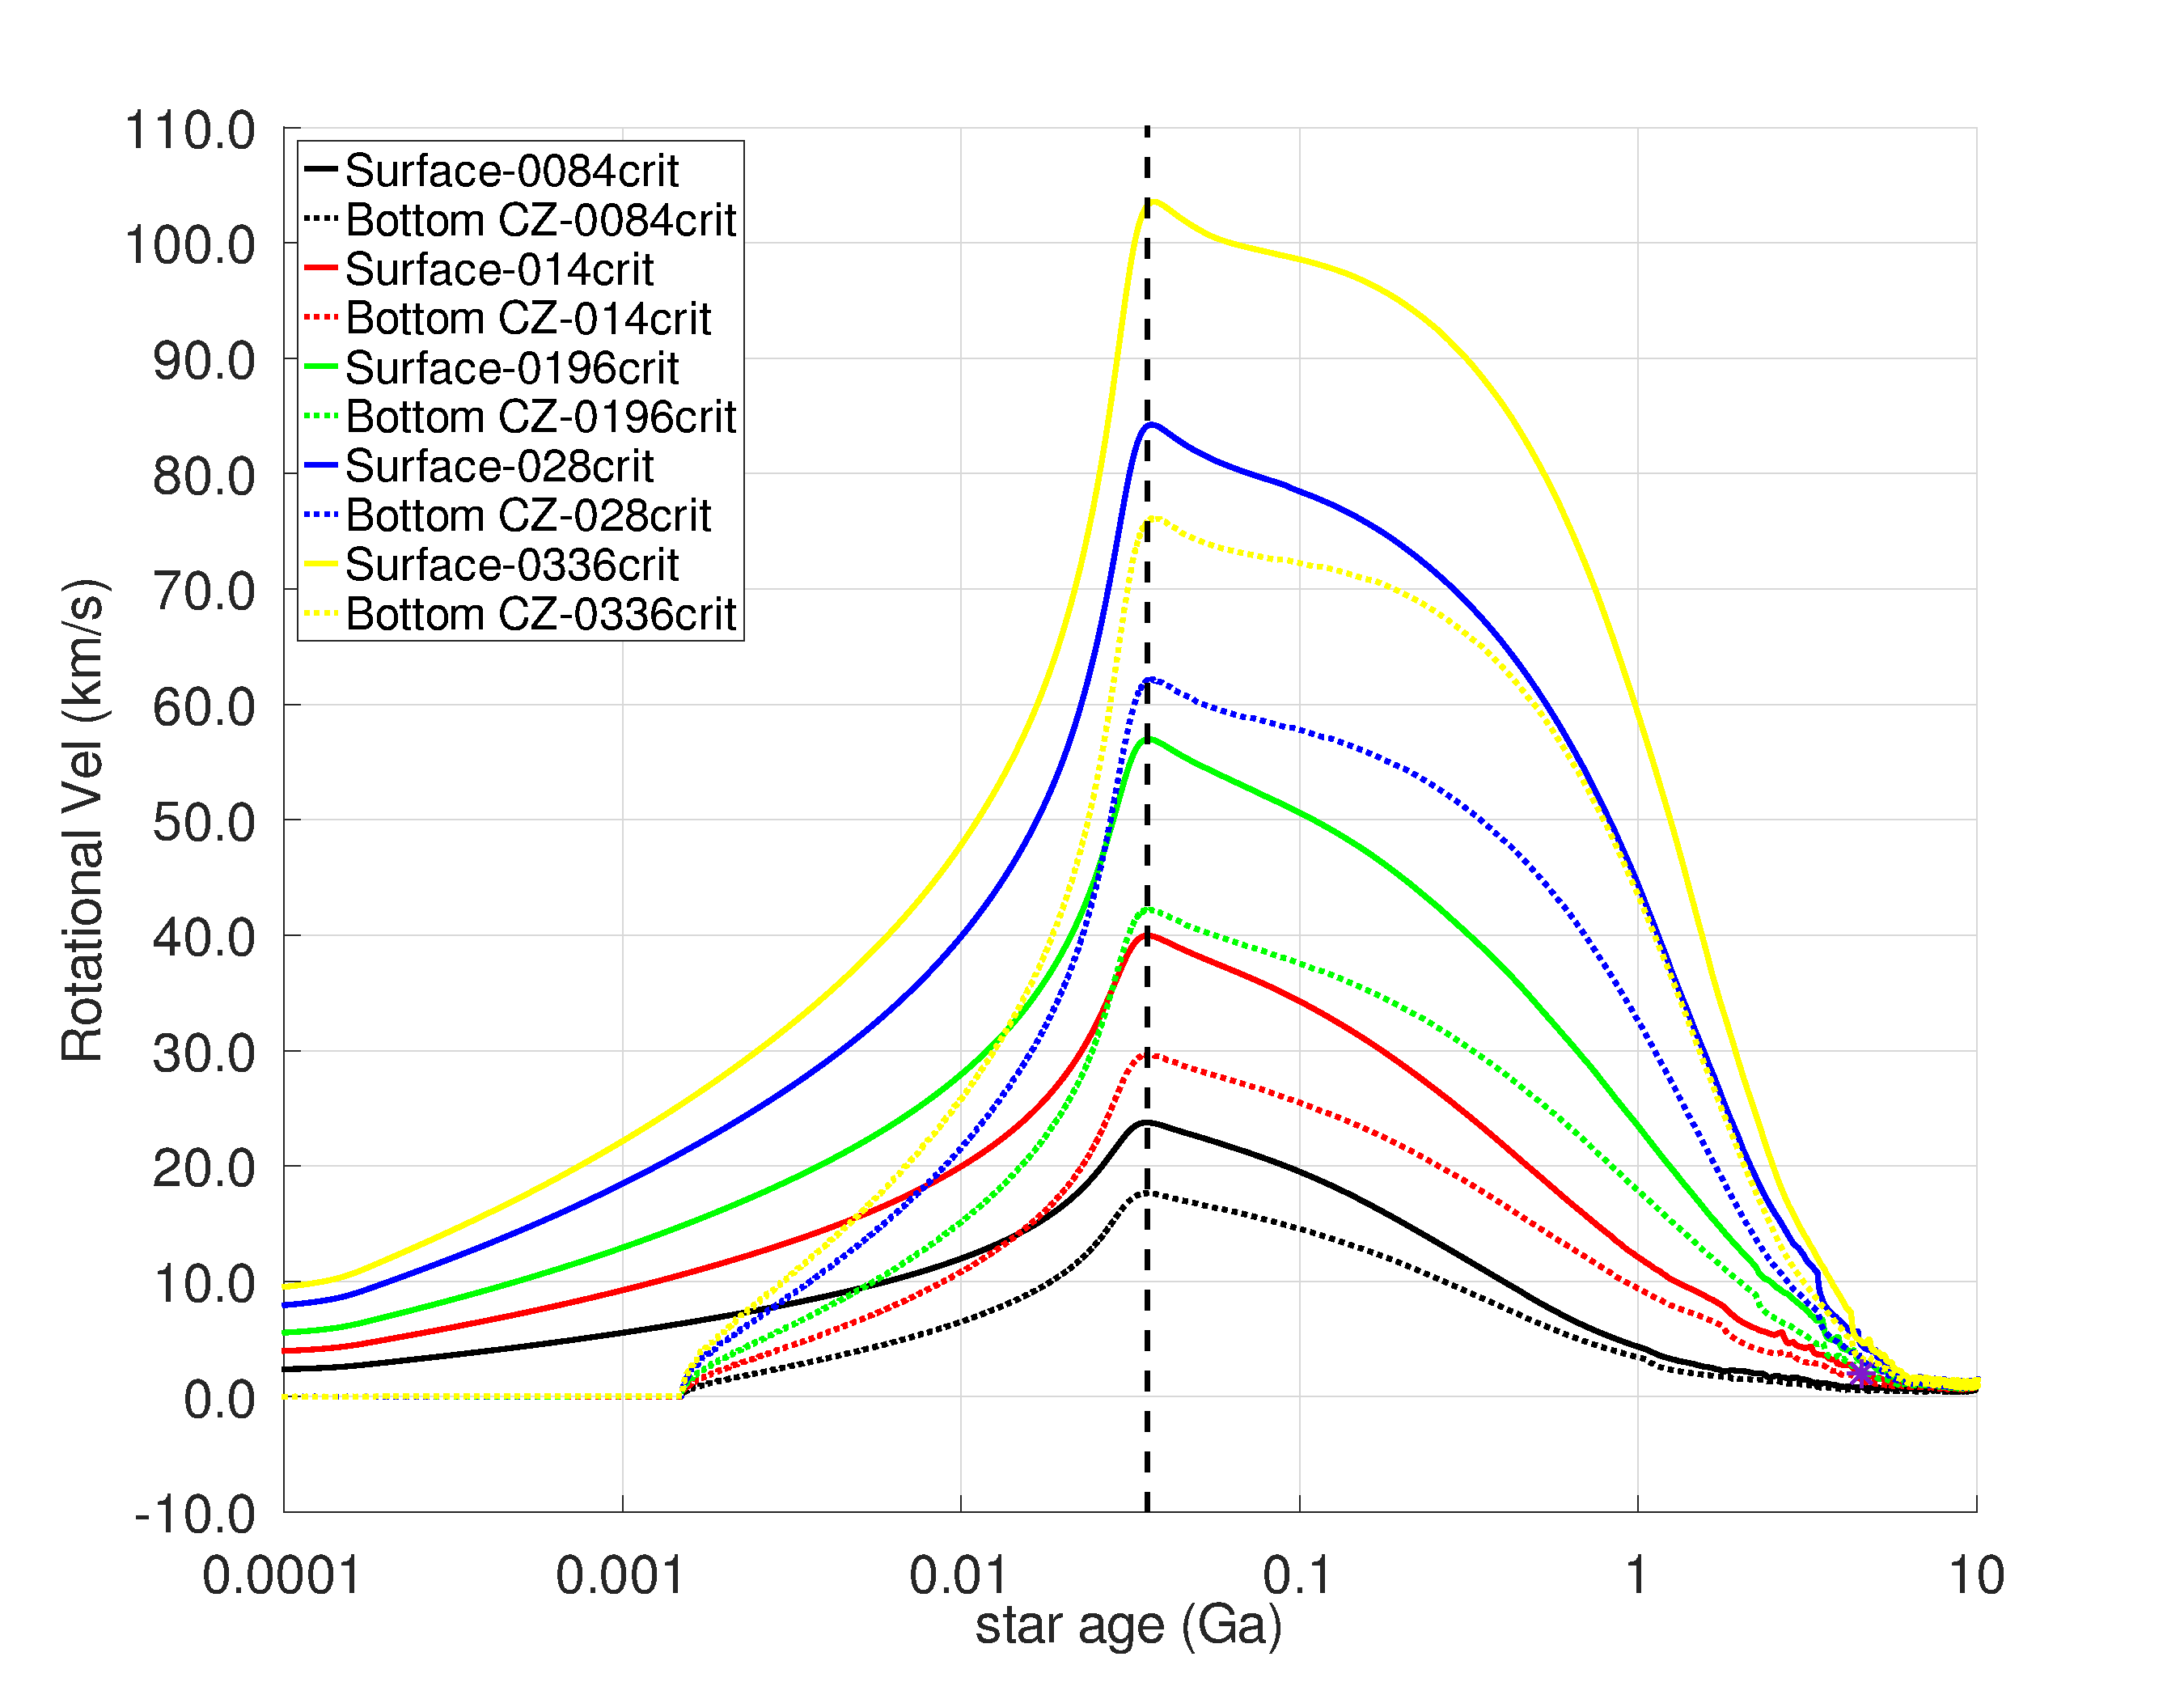
\includegraphics[width=0.7\textwidth]{img/paper2/rot_vel_var_vel_4_0g4.pdf}
	\caption{La evolución de la velocidad de rotación de la superficie, en función del tiempo para varios modelos de 1 $\msun$. Los modelos incluyen un campo magnético con una intensidad de 4G, rotación inicial con $\omegaini$ entre 0.0084 y 0.0336, respectivamente y MB. La estrella púrpura es la velocidad angular superficial para el Sol actual \cite{Gill2012}. La línea vertical discontinua hace referencia a la ZAMS.}
	\label{fig:rot_vel_var_vel_4_0g4}
\end{figure}

\subsection{Comparación con Gossage et al. (2021)}
Debido a la existencia de similitudes entre el trabajo de \cite{Gossage2021} y éste, procedemos a realizar una comparación entre ambos. Entre las similitudes encontramos el hecho de que ambos trabajos se centran en el frenado magnético, haciendo uso de MESA para las simulaciones. Entre las principales diferencias se encuentra que nuestros modelos incorporan una variable $B$ y $\amlt$. Finalmente, ambos comparan sus resultados de simulación (periodos de rotación y abundancias de Li) con arranques localizados en OCs.\par

En \cite{Gossage2021}, los autores también abordan el problema de AML desde un punto de partida similar al nuestro, pero con algunas variaciones notables. En la Tabla \ref{tab:gassage_vs_navarro} comparamos las similitudes y diferencias entre ambos estudios. En ambos trabajos los modelos consideran la rotación no sólo en el MS sino también en el PMS, con la distinción de que en el trabajo de Gossage tienen en cuenta el bloqueo del disco. Este aspecto no es tan relevante en nuestras simulaciones ya que nos hemos centrado en los perfiles de A(Li) y el trabajo de Gossage se centra principalmente en modelar los perfiles de rotación de las estrellas, que se ven afectados de forma significativa por el mecanismo de bloqueo del disco. Del mismo modo, también se consideran los efectos del frenado magnético en la pérdida de momento angular, en nuestro caso para estrellas con 1$\msun$ (gemelas-solares) y en el suyo con 0.1$\msun$$le$$\mstar$$\le$1.3$\msun$. Ambos modelos utilizan también MLT, pero en nuestro caso el valor $\amlt$ no está prefijado, sino que varía a lo largo de la simulación.\par

Estos dos trabajos se complementan ya que se basan en formalismos diferentes. Por un lado, nuestro trabajo se basa en la propuesta de \cite{Gallet2013} cuyos parámetros más relevantes son $\rossby$ y la presencia de un campo magnético de intensidad variable (B), mientras que Gossage presenta dos formalismos: \cite{Matt2015} y \cite{Garraffo2018}. El primero se caracteriza principalmente por $\rossby$ y la $\mstar$, mientras que el segundo por $\rossby$ y un parámetro que da cuenta de la complejidad de los campos magnéticos, siendo igual a 1 para un campo dipolar y mayor para multipolos de orden superior. En cuanto a las observaciones de OCs, en este trabajo hemos tenido acceso a un mayor número de ellas, y hemos cubierto un rango más amplio de edades [0.001-6.761] Gyr. Por último, ambos trabajos simulan sus respectivos modelos en MESA pero utilizando versiones diferentes.\par

\cite{Gossage2021} consiguen reproducir con mayor precisión el perfil de rotación del Sol a su edad actual \cite[ver][panel (a) de las Figuras 2, 4 \& 6]{Gossage2021} aunque como describen los autores del trabajo, calibraron sus modelos para ello, incluyendo un parámetro adicional libre de difusión ($v_0$). En nuestro trabajo, nuestro modelo no incluye este tipo de parametrización adicional y sigue siendo capaz de reproducir una velocidad de rotación ecuatorial de 4.72 km/s, un valor no especialmente alejado del valor nominal establecido de 2.0 km/s. En lo que respecta a A(Li), su modelo no consigue reproducir el valor para estrellas similares al Sol, incluido el propio Sol \cite[ver][panel (d) en las Figuras 2 \& 4, y (b) en la Figura 6]{Gossage2021}. Recalibrando algunos de los parámetros de su modelo y/o incorporando mecanismos adicionales que contribuyan a la destrucción del Li, los autores esperan obtener valores en línea con los datos observacionales. En nuestro caso (véase la sección \ref{sec_conclusiones}) pudimos reproducir A(Li) con mayor precisión.

\begin{table}
	\centering
	\begin{threeparttable}
		\begin{tabular}{lll} 
			\hline
			Parameter & This work & \cite{Gossage2021}\\
			\hline
			
			Rotation & At PMS \& MS & At PMS \& MS\\
			Solar Mass & $\mstar$=1$\msun$ & 0.1$\msun$$\le$$\mstar$$\le$1.3$\msun$ \\
			Convection & MLT variable $\alpha_{\textrm{MLT}}$ & MLT fixed $\alpha_{\textrm{MLT}}$\\
			Magnetic Braking & \cite{Gallet2013} & \cite{Matt2015}, \\ Formalism & & \cite{Garraffo2018}\\
			Magnetic Field & B(G) variable & B(G) pre-set\\ Strength & & \\
			Disk locking & Not present & Present\\
			Number of OC's & 64 & 11 \\
			Source of data & GDR3.0 GES DR5.0 & Several works \\
			MESA version & r10398 & r11701\\
			\hline
		\end{tabular}
	\end{threeparttable}
	\caption{Comparison with \cite{Gossage2021} work.}
	\label{tab:gassage_vs_navarro}    
\end{table}

\section{Conclusiones y trabajos futuros} \label{sec_conclusions}
Hemos demostrado, a través de los diferentes modelos estelares simulados, que los efectos inducidos por la combinación de ambos mecanismos de rotación y frenado magnético ofrecen una forma plausible de reconciliar los datos observacionales con los modelos teóricos. Proponemos que este resultado podría alcanzarse mediante una ley de interdependencia entre $\Omega$ y $B$. A diferencia de nuestro trabajo anterior, estos nuevos modelos eliminan las restricciones de preestablecer valores iniciales y fijos a lo largo de su evolución temporal para la intensidad del campo magnético y el parámetro $\amlt$. Hemos contrastado los resultados de los modelos con las medidas obtenidas por las misiones Gaia y GES para estrellas de características similares a nuestro Sol, centrándonos en sus abundancias de Li.\par

Nuestros modelos parecen sugerir un límite inferior a las abundancias superficiales de Li de 1.133 dex para estrellas similares al Sol, valor que se encuentra dentro del margen de error obtenido para el Sol (1.1 $\pm$ 0.1 dex). Por otro lado, predicen una velocidad de rotación en el ecuador (4.72 km/s) superior a la del Sol (2,0 km/s), por lo que podrían quemar más Li y reproducir finalmente los reservorios de Li existentes en el Sol. Junto con esta mayor velocidad angular, se desarrollaron fuertes campos magnéticos que desencadenaron un intenso frenado magnético que ralentizó su velocidad angular, pero no lo suficiente como para igualar el valor $\Omega$ actual del Sol. Además, hay que señalar que nuestros modelos no reproducen la intensidad media del campo magnético del Sol.\par

Aunque hemos mostrado cómo tanto una intensidad de campo magnético en evolución como una parametrización MLT podrían producir resultados acordes con las observaciones, debemos analizar los resultados obtenidos con cautela y no extraer conclusiones prematuras. A pesar de estas deficiencias, podemos extraer la siguiente conclusión del presente trabajo:

\begin{enumerate}
	\item Un campo magnético con intensidad variable es una alternativa válida a los modelos con un valor prefijado, ya que producen resultados en línea con trabajos anteriores para la historia rotacional de estrellas similares al Sol.
	\item Un formalismo $\amlt$ adaptativo variable podría eliminar la necesidad de prefijar su valor. Utilizándolo, pudimos reproducir valores en línea con trabajos anteriores. Además, también podría servir para derivar un intervalo de valores potenciales en los casos en que un valor por adelantado $\amlt$ es desconocido o incluso no deseable.
	\item Nuestros modelos parecen sugerir un límite inferior para A(Li)=1.133 dex a las observaciones proporcionadas por Gaia y GES para estrellas gemelas solares.   
	\item Aunque los modelos en el presente trabajo se inicializan a valores $\omegaini$ más altos que en nuestro trabajo anterior, 0.1425 y 0.0336 respectivamente, lo que resulta en $B$ hasta 3 órdenes de magnitud más intensos, $\approx$ 1KG frente a 4G, la simulación en ambos trabajos acaba produciendo valores muy similares tanto para la velocidad rotacional como para el A(Li). En el primer caso, esto se explica porque una mayor intensidad de campo magnético implica un efecto MB intensivo. Para el segundo, los valores $\amlt$ más bajos producidos por el formalismo adaptativo preservan un mayor depósito de Li durante el PMS.
\end{enumerate}


Nos gustaría concluir con las siguientes reflexiones para los próximos pasos. Es imperativo aumentar nuestra comprensión de los interiores estelares y los mecanismos de agotamiento del Li para la muestra de gemelos solares con el fin de realizar comparaciones más precisas. Además, ampliar el rango de masas en nuestros modelos nos permitirá confrontar los resultados con un rango más amplio de observaciones. Es un hecho que nuestros modelos siguen destruyendo demasiado Li al comparar los valores simulados con los de Gaia y GES.\par 

Tomando como punto de partida que las estrellas de rotación más rápida destruyen más Li, son necesarios otros mecanismos, además del MB, para explicar los datos observacionales. Entre ellos, el bloqueo al disco protoestelar podría contribuir a contrarrestar la aceleración de la estrella durante el PMS. De este modo, actuarían dos mecanismos de frenado a diferentes edades de la estrella. El bloqueo del disco actuaría durante la PMS y el MB principalmente durante la MS. Con este enfoque se establecería un mecanismo de autorregulación sobre la velocidad angular de la estrella que acabaría influyendo directamente tanto en la evolución del Li como en la intensidad del campo magnético. Para esta última se esperan intensidades menores que finalmente podrían converger con la de nuestro Sol.\par

Por otro lado, una menor velocidad de rotación también implica una menor destrucción de Li para nuestros modelos. Una forma de compensar este menor Li remanente es recurrir al over-shooting (ver \cite{Caballero2020}) un efecto que no ha sido simulado en nuestros modelos. Activando este mecanismo, permitiríamos que el Li fuera alcanzado por burbujas de material lo suficientemente calientes como para destruirlo, contribuyendo así a disminuir su abundancia. Lo ideal, como hemos hecho con $\amlt$, sería no introducir el overshooting como un parámetro fijo, sino dependiente de otros parámetros estelares fundamentales.\par


\endinput
%--------------------------------------------------------------------
% FIN DEL CAPÍTULO. 
%--------------------------------------------------------------------